\documentclass[10pt, a4paper]{article}
\usepackage{geometry}
\geometry{a4paper,total={6in, 8in}, margin=0.25in}
\usepackage{booktabs}
\usepackage{courier}
\usepackage{amssymb}
\usepackage{fourier}
\usepackage{color}
\usepackage{graphicx}
\DeclareGraphicsExtensions{.png}
\usepackage{tikz}
\usetikzlibrary{arrows}
\usetikzlibrary{shapes}

\begin{document}

\begin{enumerate}
\item\mbox{}
    \begin{enumerate}
    \item\mbox{}
        The difference between degree centrality and eigenvector centrality is that degree centrality counts the links of a node, but eigenvector centrality counts the number of neighbors of a node. In the calculation perspective, the eigenvector centrality needs to compute recursively, and it will reach an equilibrium at the end. Since we are just adding things up, the numbers would keep getting bigger, but we could reach a point where the share of the total at each node would remain stable. The shortcut to calculate such equilibrium is to find the eigenvectors and eigenvalues of the adjacency matrix A.\\
        $\mbox{A}\vec{x} = \lambda\vec{x}$\\
        In general, there will be many different eigenvalues $\lambda$ for which an eigenvector solution exists. However, the additional requirement that all the entries in the eigenvector be positive implies that only the greatest eigenvalue results in the desired centrality measure.\\

        PageRank is a variant of the eigenvector centrality measure. PageRank considers the degree of neighbors as eigenvector centrality does, but PageRank takes the outdegree of a node to consideration, the more outdegree links a node has, the node it points to would share less centrality from it. For example, if a node $v_j$ has $L\left(v_j\right)$ outgoing links, then all nodes node $v_j$ points to will share the PageRank from node $v_j$, which means that we need to divide it by $L\left(v_j\right)$. The equation is as follows:\\
        $PR\left(v_i\right) = \frac{1-d}{N} + d \displaystyle\sum_{v_j \in M\left(v_i\right)} \frac{PR\left(v_j\right)}{L\left(v_j\right)}$\\
        where $d$ is the damping factor, $v_i$ is the $i_{th}$ node under consideration, $M\left(v_i\right)$ is the set of nodes that link to $v_i$, $L\left(v_j\right)$ is the number of outbound links on node $v_j$, and $N$ is the total number of nodes.\\
        In matrix notation:\\
        $\vec{R}\left(t + 1\right) = d\mbox{A}\mbox{D}^{-1}\vec{R}\left(t\right) + \frac{1 - d}{N}\vec{1}$\\
        where D is a diagonal matrix with $\mbox{D}_{ii} = max(l_j^{out}, 1)$, and $l_j^{out}$ is the outdegree of node $v_j$\\
        For $t \rightarrow \infty$,\\
        $\vec{R} = d\mbox{A}\mbox{D}^{-1}\vec{R} + \frac{1 - d}{N}\vec{1}$\\
        $\Rightarrow \vec{R} = \mbox{D}\left(\mbox{D} - d\mbox{A}\right)^{-1}\frac{1 - d}{N}\vec{1}$\\

        HITS introduces two scores, which are authority score and hub score, but PageRank only use one score. The key differences between PageRank and HITS algorithms are HITS algorithms needs to compute two scores recursively.\\
        For HITS algorithms, if the adjacency matrix A defines as $A_{ij} = 1$ if there is an edge from $j$ to $i$; 0 otherwise, then the equation is as follows:\\
        $\left\{
            \begin{array}{lll}
                \vec{a}_k & = & \mbox{A}\vec{h}_{k-1}\\
                \vec{h}_k & = & \mbox{A}^T\vec{a}_{k-1}\\
            \end{array}
        \right.$\\
    \item\mbox{}
        Erd{\H o}s-R{\' e}nyi (ER) random graph model is obtained by starting with a set of $N$ vertices and adding adges between them at random, which denoted as $G\left(N, p\right)$, in which every possible edge occurs independently with probability $p$. In ER model, a graph in $G\left(N, p\right)$ has on average $C_2^{n}p$ edges. The distribution of the degree of any particular vertex is binomial:\\
        $P\left(deg\left(v\right) = k\right) = C_k^{N-1}p^k\left(1 - p\right)^{N-1-k}$\\
        where $N$ is the total number of vertices in the graph.\\
        The distribution is Poisson for large $N$ and $Np = const$:\\
        $P\left(deg\left(v\right) = k\right) \rightarrow \frac{\left(Np\right)^ke^{-Np}}{k!}$ as $N \rightarrow \infty$ and $Np = const$\\

        The ER graphs fail to explain two important properties observed in real-world networks, but Watts-Strogatz small world model does. The two properties are:
        \begin{itemize}
        \item By assuming a constant and independent probability of two nodes being connected, they do not account for local clustering, which results in a low clustering coefficient.
        \item Do not account for the formation of hubs. Formally, the degree distribution of ER graphs converges to a Poisson distribution, rather than a power law observed in most real-world, scale-free networks.
        \end{itemize}
        Watts small world model has small diameter and is high clustering.\\

        Limitation of Watts-Strogatz model is that the model produces graphs that are homogeneous in degree, but real networks are often inhomogeneous in degree, having hubs and a scale-free degree distribution. In contrast, Barab{\' a}si-Albert (BA) model is a scale-free network because it assumes that edges from the new vertex are more likely to link to nodes with higher degrees, and it results in a network whose degree distribution follows a power law, at least asymptotically.\\

        Preferential attachment means that the more connected a node is, the more likely it is to receive new links. Preferential attachment method:\\
        Start with two vertices connected by an edge\\
        for $i = 3$ to $N$\\
        \-\hspace{1em} for each $1 <= j < i$, $d\left(j\right) = $degree of vertex $j$ so far\\
        \-\hspace{2em} let $Z = \sum d\left(j\right)$ (sum of all degrees so far)\\
        \-\hspace{2em} add new vertex $i$ with $k$ edges back to $\left\{1, ..., i - 1\right\}$:\\
        \-\hspace{3em} $i$ is connected back to $j$ with probability $d\left(j\right) / Z$
    \end{enumerate}
\item\mbox{}
    \begin{enumerate}
    \item\mbox{}
        The concept of RankClus is that ranking and clustering can mutual enhance each other. The higher the ranking score in a cluster, the higher probability the node plays an important role in that cluster, and vice versa. In contrast, SimRank-based clustering is a simple ranking method that doesn't consider the weight for each node in the network. It will create an unfair result while each node actually has different weight.\\

        RankClus just need to compare distance with all cluster center for each iteration, while SimRank needs to calculate the distance of nodes by the similarity. It gets the similarity by checking all the neighbors' similarity, and the neighbors' similarity are calculated also by checking all their neighbors. So actually it needs to traverse the whole network to calculate the similarity between two nodes. That's why RankClus is more efficient than SimRank.\\
        SimRank will be at least quadratic at each iteration since it evaluates distance between every pair in the network. Therefore, the complexity of SimRank is $\Omega\left(|V|^2\right)$\\
        In each iteration, RankClus has time complexity as follows:
        \begin{itemize}
        \item Ranking for sparce network: $\sim O\left(|E|\right)$
        \item Mixture model estimation: $\sim O\left(K|E| + mK\right)$
        \item Cluster adjustment: $\sim O\left(mK^2\right)$
        \end{itemize}
        In all, linear to $|E| \Rightarrow \sim O\left(K|E|\right)$
    \item\mbox{}
        \begin{enumerate}
            \item $A - P - A$, which means that two authors are close collaborators\\
                The authors collaborate together will be in the same cluster
            \item $A - P - V - P - A$, which means that two authors work on similar topics and have similar reputation
                The authors work on similar topics and have similar reputation will be in the same cluster
            \item $A - P \rightarrow P \leftarrow P - A$, which means that papers from two authors cite the same paper
                The authors publishing papers cite the same papers will be in the same cluster
        \end{enumerate}
        A user can first create some examples for the way they want to cluster, such as who should be clustered with whom. After that, we can first analyze the structure of these examples, and then find meta-paths that can cluster nodes closer to the given examples. Then we can use these meta-paths to perform clustering, and it should get similar clustering results just like the form of the user-given examples.
    \end{enumerate}
\item\mbox{}
    \begin{enumerate}
    \item\mbox{}\\
        \begin{tabular}{ll}
            TI: & Title (paper)\\
            AD: & Affiliation\\
            AU: & Author\\
            AB: & Abstract\\
            SO: & Source (venue)\\
            TE: & Term\\
        \end{tabular}\\
        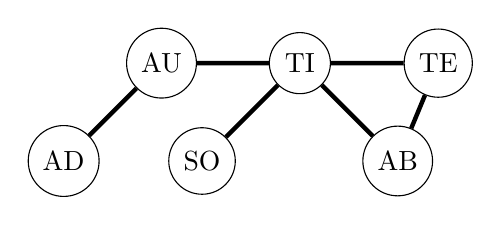
\begin{tikzpicture}
            \tikzstyle{main node}=[draw,auto,node distance=50pt,circle,align=center]
            \node[main node] (AU) {AU};
            \node[main node] (AD) [below left of=AU] {AD};
            \node[main node] (TI) [right of=AU] {TI};
            \node[main node] (SO) [below left of=TI] {SO};
            \node[main node] (AB) [below right of=TI] {AB};
            \node[main node] (TE) [right of=TI] {TE};

            \draw[ultra thick]
                (TI) -- (AB)
                (TI) -- (AU)
                (AD) -- (AU)
                (TI) -- (SO)
                (TI) -- (TE)
                (AB) -- (TE);
        \end{tikzpicture}

        Example 1:\\
        AU -- TI -- AU, which means that two authors are close collaborators\\
        Example 2:\\
        AU -- TI -- AB -- TI -- AU, which means that two authors work on similar topic
    \item\mbox{}\\
        Classify articles according to the medicine the article is focusing on.\\
        We can apply a modified RankClass algorithm to classify articles according to the medicine the article is focusing on. First, we can determine several different categories, such as penicillin, medical marijuana, and steroid. Second, initialize each article different ranking score based on the normalized count of the medicine appears in the title and abstract. Third, update ranking score of each object recursively by looking at the ranking of its neighbors. When the ranking score converges, we can determine the class of each article by selecting the highest ranking score among all classes.\\
    \end{enumerate}

\item\mbox{}
    \begin{enumerate}
    \item\mbox{}\\
        In heterogeneous network, we can perform schema-guided relationship prediction to explore semantic relationships among similar typed links. That's why using hetergeneous network is better. We can find meta-paths with high significance level, and it can be great topological features to help us predict new co-authors. In addition, the hybrid measure of path count, normalized path count, random walk, and symmetric random walk also improve the accuracy of the prediction.
    \item\mbox{}\\
        %With the database, we can get the content of the paper which is cited by the input paper. First, find papers having similar schema with the input paper, the selected papers would be good predictions that
        $\mbox{P}\rightarrow\mbox{P}$, which means that a paper cites another paper\\
        $\mbox{P}\rightarrow\mbox{P}\leftarrow\mbox{P}$, which means that two papers cite the same paper\\
        All of these meta-paths have influence on the probability of referencing paper, and we can use hybrid measurement of normalized path count, path count, random walk, and symmetric random walk to measure the values of these meta-paths.\\
        After that, for each paper in the dataset, we could train a model to classify whether the paper should be cited or not by the input paper. Because the meta-path contains semantic meaning of topological features, good meta-paths and measure should help us output quality results.
    \end{enumerate}

\end{enumerate}

\end{document}
